\documentclass[11pt,a4paper]{article}
\usepackage[margin=2.5cm]{geometry}
\usepackage{booktabs}
\usepackage{amsmath}
\usepackage{hyperref}
\usepackage{pgfplots}
\pgfplotsset{compat=1.18}
\usepackage{array}
\usepackage{parskip}

\hypersetup{colorlinks=true, linkcolor=blue, urlcolor=blue}

\title{\textbf{IEEE 30-Bus Battery Siting --- Model Reference}}
\author{}
\date{}

\begin{document}
\maketitle
\tableofcontents
\newpage

% ============================================================
\section{Use Case Overview}

\begin{itemize}
  \item \textbf{Network:} IEEE 30-bus, 41 branches, 6 generators (MATPOWER case30)
  \item \textbf{Batteries:} 4 units (30 MW / 120 MWh each), placement to be optimised
  \item \textbf{Search space:} $\binom{30}{4} = 27{,}405$ candidate placements
  \item \textbf{Objective:} minimise total 24-hour system dispatch cost
  \item \textbf{Horizon:} single 24-hour day, hourly resolution
  \item \textbf{Power flow:} DC approximation (PTDF-based, lossless, no reactive power)
  \item \textbf{Quantum siting:} 6 gen qubits + 30 bus qubits = \textbf{36 qubits} (Aer TN recommended)
  \item \textbf{Source:} \url{https://github.com/Square-Peg-Technologies/square-peg-quantum-challenge}
\end{itemize}

\subsection*{Key Files and Variables}

\begin{tabular}{@{}lll@{}}
\toprule
File & Variable / Function & Description \\
\midrule
\texttt{ieee30.py} & \texttt{Case} & Grid object: PTDF, fbar, power\_demand \\
 & \texttt{Case.factors} & 24-hour demand multipliers (list of 24) \\
 & \texttt{CaseDescription.fbar} & Branch flow limits (MW), 41 elements \\
 & \texttt{CaseDescription.branch} & Branch r, x, b, ratio data \\
 & \texttt{CaseDescription.bus} & Bus Pd, Qd base values \\
\texttt{assets.py} & \texttt{GENERATORS} & List of 6 generator dicts (bus, Pmin, Pmax, cost) \\
 & \texttt{BATTERIES} & List of 4 battery dicts (power\_mw, capacity\_mwh, \ldots) \\
 & \texttt{DATACENTER\_BUS} & None (base case, no datacenter) \\
 & \texttt{DATACENTER\_MW} & 0.0 (base case) \\
\texttt{locations.py} & \texttt{GENERATOR\_LOCATIONS} & Dict \{gen\_index: bus\} \\
 & \texttt{BATTERY\_LOCATIONS} & Placeholder; overridden by solver \\
\texttt{case30.m} & --- & MATPOWER source data (retrieved June 2026) \\
\bottomrule
\end{tabular}

% ============================================================
\section{Network: IEEE 30-Bus}

\subsection{Bus Data}

\begin{tabular}{@{}rllrrl@{}}
\toprule
Bus & Type & Base Pd (MW) & Base Qd (MVAr) & Notes \\
\midrule
1  & Slack (3) &  0.0 &  0.0 & Generator only \\
2  & PV (2)    & 21.7 & 12.7 & Generator + load \\
3  & PQ (1)    &  2.4 &  1.2 & Load only \\
4  & PQ (1)    &  7.6 &  1.6 & Load only \\
5  & PQ (1)    &  0.0 &  0.0 & Shunt cap 0.19 pu \\
6  & PQ (1)    &  0.0 &  0.0 & Transit bus \\
7  & PQ (1)    & 22.8 & 10.9 & Load only \\
8  & PQ (1)    & 30.0 & 30.0 & Load only \\
9  & PQ (1)    &  0.0 &  0.0 & Transit bus \\
10 & PQ (1)    &  5.8 &  2.0 & Load only \\
11 & PQ (1)    &  0.0 &  0.0 & Transit bus \\
12 & PQ (1)    & 11.2 &  7.5 & Load only \\
13 & PV (2)    &  0.0 &  0.0 & Generator only \\
14 & PQ (1)    &  6.2 &  1.6 & Load only \\
15 & PQ (1)    &  8.2 &  2.5 & Load only \\
16 & PQ (1)    &  3.5 &  1.8 & Load only \\
17 & PQ (1)    &  9.0 &  5.8 & Load only \\
18 & PQ (1)    &  3.2 &  0.9 & Load only \\
19 & PQ (1)    &  9.5 &  3.4 & Load only \\
20 & PQ (1)    &  2.2 &  0.7 & Load only \\
21 & PQ (1)    & 17.5 & 11.2 & Load only \\
22 & PV (2)    &  0.0 &  0.0 & Generator only \\
23 & PV (2)    &  3.2 &  1.6 & Generator + load \\
24 & PQ (1)    &  8.7 &  6.7 & Shunt cap 0.04 pu \\
25 & PQ (1)    &  0.0 &  0.0 & Transit bus \\
26 & PQ (1)    &  3.5 &  2.3 & Load only \\
27 & PV (2)    &  0.0 &  0.0 & Generator only \\
28 & PQ (1)    &  0.0 &  0.0 & Transit bus \\
29 & PQ (1)    &  2.4 &  0.9 & Load only \\
30 & PQ (1)    & 10.6 &  1.9 & Load only \\
\midrule
\multicolumn{2}{@{}l}{\textbf{Total base load}} & \textbf{189.2} & & \\
\bottomrule
\end{tabular}

\subsection{Branch Data}

\begin{tabular}{@{}rllrrrrl@{}}
\toprule
Br\# & From--To & r (pu) & x (pu) & b (pu) & Limit (MW) & Ratio & Note \\
\midrule
 0 & 1--2   & 0.0200 & 0.0600 & 0.0300 & 130 & -- & Strong backbone \\
 1 & 1--3   & 0.0500 & 0.1900 & 0.0200 & 130 & -- & \\
 2 & 2--4   & 0.0600 & 0.1700 & 0.0200 &  65 & -- & \\
 3 & 3--4   & 0.0100 & 0.0400 & 0.000  & 130 & -- & \\
 4 & 2--5   & 0.0500 & 0.2000 & 0.0200 & 130 & -- & \\
 5 & 2--6   & 0.0600 & 0.1800 & 0.0200 &  65 & -- & \\
 6 & 4--6   & 0.0100 & 0.0400 & 0.000  &  90 & -- & \\
 7 & 5--7   & 0.0500 & 0.1200 & 0.0100 &  70 & -- & \\
 8 & 6--7   & 0.0300 & 0.0800 & 0.0100 & 130 & -- & \\
 9 & 6--8   & 0.0100 & 0.0400 & 0.000  &  32 & -- & Bottleneck to bus-8 cluster \\
10 & 6--9   & 0.0000 & 0.2100 & 0.000  &  65 & -- & \\
11 & 6--10  & 0.0000 & 0.5600 & 0.000  &  32 & -- & High-x path \\
12 & 9--11  & 0.0000 & 0.2100 & 0.000  &  65 & -- & \\
13 & 9--10  & 0.0000 & 0.1100 & 0.000  &  65 & -- & \\
14 & 4--12  & 0.0000 & 0.2600 & 0.000  &  65 & -- & \\
15 & 12--13 & 0.0000 & 0.1400 & 0.000  &  65 & -- & \\
16 & 12--14 & 0.1200 & 0.2600 & 0.000  &  32 & -- & \\
17 & 12--15 & 0.0700 & 0.1300 & 0.000  &  32 & -- & \\
18 & 12--16 & 0.0900 & 0.2000 & 0.000  &  32 & -- & \\
19 & 14--15 & 0.2200 & 0.2000 & 0.000  &  16 & -- & Weak peripheral link \\
20 & 16--17 & 0.0800 & 0.1900 & 0.000  &  16 & -- & \\
21 & 15--18 & 0.1100 & 0.2200 & 0.000  &  16 & -- & \\
22 & 18--19 & 0.0600 & 0.1300 & 0.000  &  16 & -- & \\
23 & 19--20 & 0.0300 & 0.0700 & 0.000  &  32 & -- & \\
24 & 10--20 & 0.0900 & 0.2100 & 0.000  &  32 & -- & \\
25 & 10--17 & 0.0300 & 0.0800 & 0.000  &  32 & -- & \\
26 & 10--21 & 0.0300 & 0.0700 & 0.000  &  32 & -- & \\
27 & 10--22 & 0.0700 & 0.1500 & 0.000  &  32 & -- & \\
28 & 21--22 & 0.0100 & 0.0200 & 0.000  &  32 & -- & \\
29 & 15--23 & 0.1000 & 0.2000 & 0.000  &  16 & -- & \\
30 & 22--24 & 0.1200 & 0.1800 & 0.000  &  16 & -- & \\
31 & 23--24 & 0.1300 & 0.2700 & 0.000  &  16 & -- & \\
32 & 24--25 & 0.1900 & 0.3300 & 0.000  &  16 & -- & \\
33 & 25--26 & 0.2500 & 0.3800 & 0.000  &  16 & -- & Peripheral feeder \\
34 & 25--27 & 0.1100 & 0.2100 & 0.000  &  16 & -- & \\
35 & 28--27 & 0.0000 & 0.4000 & 0.000  &  65 & -- & \\
36 & 27--29 & 0.2200 & 0.4200 & 0.000  &  16 & -- & \\
37 & 27--30 & 0.3200 & 0.6000 & 0.000  &  16 & -- & High-x tail \\
38 & 29--30 & 0.2400 & 0.4500 & 0.000  &  16 & -- & \\
39 & 8--28  & 0.0600 & 0.2000 & 0.0200 &  32 & -- & \\
40 & 6--28  & 0.0200 & 0.0600 & 0.0100 &  32 & -- & \\
\bottomrule
\end{tabular}

Key bottlenecks: branches 9 (6--8, 32 MW), 11 (6--10, 32 MW), 19/20/21 (16 MW peripheral
feeders in the bus-14--20 cluster) bind at peak and produce non-zero shadow prices.

% ============================================================
\section{Generators}

Six generators. Two cheap units (buses 1, 2), two medium units (buses 22, 27), two expensive
units (buses 23, 13). Cost uses the MATPOWER case30 polynomial gencost
($a_g p^2 + b_g p + c_g$, with $c_g = 0$).

\begin{tabular}{@{}llrrrrl@{}}
\toprule
Name  & Bus & Pmin (MW) & Pmax (MW) & $a_g$ (\$/MW$^2$h) & $b_g$ (\$/MWh) & Startup (\$) \\
\midrule
Gen 1 &  1 & 10 &  80 & 0.02000 & 2.00 & 0 \\
Gen 2 &  2 & 10 &  80 & 0.01750 & 1.75 & 0 \\
Gen 3 & 22 & 10 &  50 & 0.06250 & 1.00 & 0 \\
Gen 4 & 27 & 10 &  55 & 0.00834 & 3.25 & 0 \\
Gen 5 & 23 &  5 &  30 & 0.02500 & 3.00 & 0 \\
Gen 6 & 13 &  5 &  40 & 0.02500 & 3.00 & 0 \\
\midrule
\multicolumn{3}{@{}l}{Total installed} & \textbf{335 MW} & & & \\
\bottomrule
\end{tabular}

Note: Pmin raised from 0 (MATPOWER default) to small positive values so that unit-commitment
decisions are meaningful. At peak demand (264.9 MW) the system has 26\% reserve.

% ============================================================
\section{Load Profile}

The 24-hour demand shape is defined in \texttt{ieee30.py} (\texttt{Case.factors}), a list of 24
hourly multipliers applied uniformly to all base bus loads. Source: synthetic daily shape scaled
to the MATPOWER case30 base load of 189.2 MW.
Peak system demand: $189.2 \times 1.40 = 264.9$ MW at Hour 13.

\begin{center}
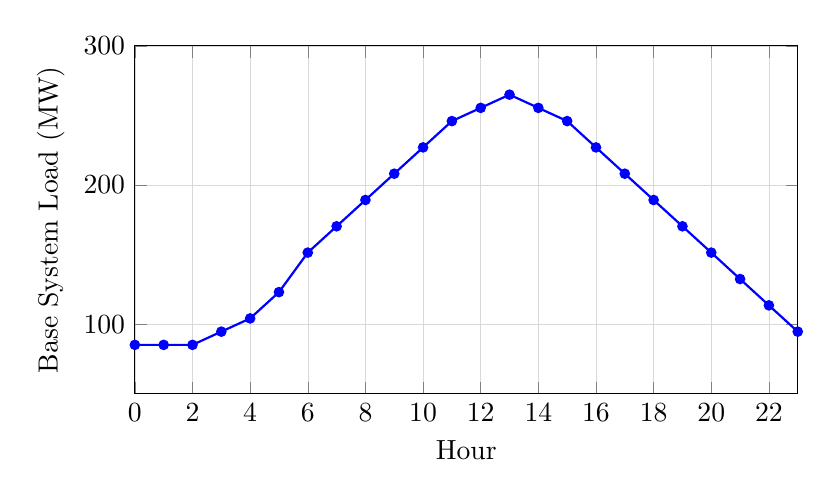
\begin{tikzpicture}
\begin{axis}[
  width=10cm, height=6cm,
  xlabel={Hour}, ylabel={Base System Load (MW)},
  xmin=0, xmax=23, ymin=50, ymax=300,
  xtick={0,2,4,6,8,10,12,14,16,18,20,22},
  grid=both, grid style={line width=0.2pt, draw=gray!30},
  mark size=1.5pt,
]
\addplot[blue, thick, mark=*] coordinates {
  (0, 85.1) (1, 85.1) (2, 85.1) (3, 94.6) (4, 104.1) (5, 123.0)
  (6, 151.4) (7, 170.3) (8, 189.2) (9, 208.1) (10, 227.0) (11, 245.9)
  (12, 255.4) (13, 264.9) (14, 255.4) (15, 245.9) (16, 227.0) (17, 208.1)
  (18, 189.2) (19, 170.3) (20, 151.4) (21, 132.4) (22, 113.5) (23, 94.6)
};
\end{axis}
\end{tikzpicture}
\end{center}

% ============================================================
\section{Battery Specifications}

Four identical batteries: \textbf{30 MW / 120 MWh, charge efficiency 90\% (discharge lossless),
initial SoC 120 MWh (fully charged).} Defined in \texttt{assets.py} as \texttt{BATTERIES}.

% ============================================================
\section{Problem Formulation}

\subsection{Objective}

The cost function in \texttt{solvers/uc.py} supports a quadratic-plus-linear form:

\[
  \min \sum_g \sum_{t=1}^{24} \left[ a_g \cdot p_{g,t}^2 + b_g \cdot p_{g,t} + c_g \cdot u_{g,t} + \mathrm{sc}_g \cdot v_{g,t} \right]
\]

In this use case all six generators carry the MATPOWER polynomial cost coefficients directly
($a_g > 0$). No-load costs $c_g$ and startup costs $\mathrm{sc}_g$ are zero.

\subsection{Decision Variables}

\begin{itemize}
  \item $p_{g,t} \ge 0$: generator output (MW)
  \item $u_{g,t} \in \{0,1\}$: generator commitment (1 = online)
  \item $v_{g,t} \in \{0,1\}$: startup indicator
  \item $r^+_{b,t} \ge 0$: battery charge (MW)
  \item $r^-_{b,t} \ge 0$: battery discharge (MW)
  \item $\mathrm{SoC}_{b,t} \ge 0$: state of charge (MWh)
  \item $z_{b,t} \in \{0,1\}$: direction flag (1 = charging)
\end{itemize}

\subsection{Constraints}

\textbf{Generator bounds:}
\[
  P_g^{\min} \cdot u_{g,t} \le p_{g,t} \le P_g^{\max} \cdot u_{g,t}
\]

\textbf{Power balance} (per hour):
\[
  \sum_g p_{g,t} + \sum_b (r^-_{b,t} - r^+_{b,t}) = \sum_i D_{i,t}
\]

\textbf{DC line flow limits} (per branch $\ell$, per hour):
\[
  -\bar{f}_\ell \le \sum_i \mathrm{PTDF}_{\ell,i} \cdot \mathrm{net}_{i,t} \le \bar{f}_\ell
\]

\textbf{Battery charge/discharge exclusion:}
\[
  r^+_{b,t} \le P^{\mathrm{bat}} \cdot z_{b,t}, \qquad r^-_{b,t} \le P^{\mathrm{bat}} \cdot (1 - z_{b,t})
\]

\textbf{SoC bounds:} $0 \le \mathrm{SoC}_{b,t} \le 120$ MWh, with $\mathrm{SoC}_{b,0} = 120$ MWh.

\subsection{Siting Algorithm}

The Benders decomposition (\texttt{siting\_benders.py}) works as follows:
\begin{enumerate}
  \item \textbf{Master problem} (SCIP MIP): selects which buses to place the 4 batteries on.
        Exactly one bus per battery; symmetry-breaking enforces ascending bus index.
  \item \textbf{Subproblem} (\texttt{run\_uc()}): given a fixed placement, solves the 24-hour UC/ED.
        Returns total cost $Z$.
  \item \textbf{Cuts:} no-good cuts prevent re-visiting placements. L-shaped optimality cuts
        $\eta \ge Z \cdot (\sum_{(b,n) \in S^+} x_{b,n} - (M-1))$ bound the master.
  \item \textbf{Convergence:} master lower bound $\ge$ best known cost, or time limit.
\end{enumerate}

An alternative joint MILP is in \texttt{siting\_mip.py} (single SCIP solve, big-M
linearisation of placement $\times$ dispatch).

% ============================================================
\section{Quantum Siting}

The quantum siting solver (\texttt{solvers/quantum\_siting.py}) encodes the joint
(generator commitment, battery placement) decision as a \textbf{36-qubit} QAOA/VQA problem.

\begin{itemize}
  \item \textbf{Qubit layout:} $u_0 \ldots u_5$ (6 generator bits) $\| s_0 \ldots s_{29}$ (30 bus bits)
  \item \textbf{Circuit:} butterfly ans\"{a}tz, $L$ layers, $2Ln$ parameters
  \item \textbf{Optimiser:} COBYLA with plateau detection (patience $= \max(50, 2Ln)$ evals)
  \item \textbf{Recommended backend:} \texttt{aer\_tn} (Aer tensor-network MPS simulator);
        statevector simulation of 36 qubits requires $\sim$1\,TB RAM and is not practical
\end{itemize}

\textbf{Proxy cost function} $Q(u, s)$ encodes:
\begin{enumerate}
  \item $c_{\min}(u)$: minimum-cost dispatch at $p_g = P_g^{\min}$ for committed generators
  \item $\lambda_1 \cdot (\sum_i s_i - B)^2$: battery-budget penalty (exactly $B$ batteries)
  \item $\lambda_2 \cdot \max(0,\, D - \sum_g P_g^{\max} u_g)^2$: generator shortfall penalty
  \item $-P_{\mathrm{loc}}(s)$: congestion relief bonus from PTDF $\times$ shadow-price signal
\end{enumerate}

% ============================================================
\section{Comparison}

\begin{tabular}{@{}llll@{}}
\toprule
Method & Solver & Qubit / binary vars & Typical runtime \\
\midrule
ED (fixed placement) & CVXPY / Clarabel & none & $<$1 s \\
UC (fixed placement) & CVXPY / SCIP & $6 \times 24 = 144$ binary & 5--30 s \\
Siting (Benders) & SCIP + UC & none (iterative) & 60--300 s \\
Siting (MIP) & SCIP & $30 \times 4 = 120$ binary & 60--600 s \\
Quantum (D-Wave SA) & dimod SA & 36 qubits (BQM) & 5--20 s \\
Quantum (Qiskit SV) & Aer statevector & 36 qubits & not practical ($\sim$1\,TB) \\
Quantum (Aer TN) & Aer MPS & 36 qubits & 60--300 s \\
\bottomrule
\end{tabular}

\end{document}
